% mainfile: ../../../../master.tex
\subsection{DNA quantification with Qubit\texttrademark~ DNA BR Assay Kit}
% The part of the label after the colon must match the file name. Otherwise,
% conditional compilation based on task labels does NOT work.
\label{task:20180301_cj2}
\tags{lab,dna,qnt}
\authors{cj}
%\files{}
%\persons{}


\begin{figure}[H] % position of the figure 
    \centering
    \caption{Illustration for the Qubit\texttrademark~ DNA BR assay}
    \label{fig:20180301_Qubit_dsDNA_BR}
    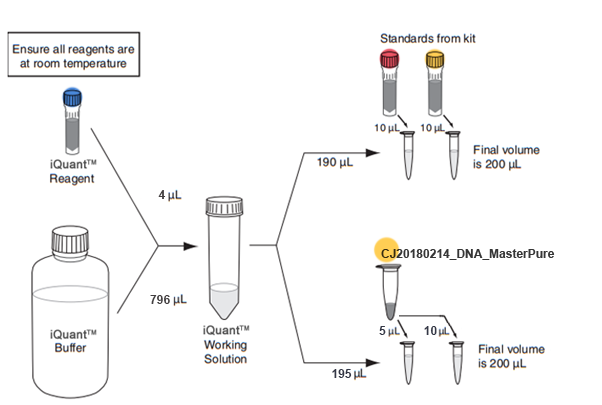
\includegraphics[width=0.8\textwidth]{graphics/schemas/20180215_Qubit_dsDNA_BR.png}
\end{figure}
\sidenote{Qubit\texttrademark DNA BR Assay Kit \texttt{LOT:\#1835789} opened by Elísabet on 20170815.}

\comment{It is exactly the same as what was done on the 20180215.}

In table \ref{tab:20180301_nuc_acid_qnt}, the quantities of DNA are calculted based on the volume left: I know I eluted my DNA with 2 x 100~\uL of Tris HCl buffer which makes it a total 200~\uL, then I used 2~\uL for the NanoDrop\cR measurments and finally I use 5~\uL and 10~\uL for the Qubit\texttrademark~ assay. Which means the volume left us 183~\uL.

\begin{table}[H]
\caption{Total DNA quantities in samples measured with Qubit\texttrademark~ DNA BR Assay Kit}
\label{tab:20180301_nuc_acid_qnt}
\centering
\begin{tabular}{l r r r r}
\toprule
Sample ID & \textmu g/mL & $V_f$ (mL) & m (\textmu g) & m (ng) \\ \midrule
\texttt{CJ20180301\_DNA\_AllPrep\_5} & 2.89 & 0.183 & 0.528 & 528.87 \\
\texttt{CJ20180301\_DNA\_AllPrep\_10} & 2.93 & 0.183 & 0.536 & 536.19 \\
\midrule
\texttt{CJ20180301\_DNA\_AllPrep\_5} & 3.52 & 0.183 & 0.461 & 461.16 \\
\texttt{CJ20180301\_DNA\_AllPrep\_10} & 3.46 & 0.183 & 0.450 & 450.18 \\
\texttt{CJ20180301\_DNA\_AllPrep\_5} & \textbf{3.45} & 0.183 & 0.448 &448.35 \\
\texttt{CJ20180301\_DNA\_AllPrep\_10} & 3.44 & 0.183 & 0.446 & 446.52 \\
\bottomrule
\end{tabular}
\end{table}

In table \ref{tab:20180301_nuc_acid_qnt}, the two first rows shows measurments obtained with the previous calibration, while the four last rows were obtained with a new calibration. I was just curious to see how measurements would compare. I think the difference in the values measured can be explained by the pipetting errors when preparing the assay.

And since the volume used to elute the DNA was 200 \uL and the concentration is at least 3.45 \textmu g/mL, the DNA yield is 690 ng. This is not enough for a \gls{pcr}-free library preparation for shotgun metagenomics, but I must keep in mind that my starting material (2~mL of culture) is very likely smaller than the one I will get from my Sterivex\texttrademark filters.

